% Define document class
% Using IEEE Transaction class and format
\documentclass[10pt,journal,compsoc]{IEEEtran}

% Define packages being used to generate typeset
\usepackage[margin=1in]{geometry}
\usepackage{graphicx}
\usepackage{textcomp}
\usepackage{csquotes}
\usepackage{stackengine}[2013-10-15]
\newcommand\textss[1]{\stackengine{.9ex}{}{\scriptsize#1}{O}{l}{F}{F}{L}}
\usepackage{url}
\usepackage{hyperref}
\usepackage{amssymb,amsmath}

% Begin Document
\begin{document}

% Document Title
\title{Contact Force Regulation at the PSM and \\Haptic Feedback at the MTM \\of the da Vinci Research Kit}

% author names and memberships
\author{Kiran~Mohan, Amit~Trivedi,~\IEEEmembership{Member,~IEEE,}  Aman~Rana, Terence~Carmichael, Akanksha~Devkar
\IEEEcompsocitemizethanks{\IEEEcompsocthanksitem A. Trivedi, Department of Robotics Engineering, Worcester Polytechnic Institute, Worcester, MA, 01609.\protect\\ E-mail: atrivedi@wpi.edu
\IEEEcompsocthanksitem K. Mohan, Department
of Robotics Engineering, Worcester Polytechnic Institute, Worcester,
MA, 01609.\protect\\
E-mail: kmohan@wpi.edu
\IEEEcompsocthanksitem A. Rana, Department
of Robotics Engineering, Worcester Polytechnic Institute, Worcester,
MA, 01609.\protect\\
E-mail: arana@wpi.edu
\IEEEcompsocthanksitem T. Carmichael, Department
of Robotics Engineering, Worcester Polytechnic Institute, Worcester,
MA, 01609.\protect\\
E-mail: twcarmichael@wpi.edu
\IEEEcompsocthanksitem A. Devkar, Department
of Electrical and Computer Engineering, Worcester Polytechnic Institute, Worcester,
MA, 01609.\protect\\
E-mail: acdevkar@wpi.edu}
\thanks{Document revised March 21, 2016.}}

% the paper headers
\markboth{RBE-501 - Team-3 Project, ~Spring 2016}%
{Shell \MakeLowercase{\textit{et al.}}: Contact Force Regulation at the PSM and Haptic Feedback at the MTM of the da Vinci Research Kit}

% Abstract
\IEEEtitleabstractindextext{%
\begin{abstract}
The purpose of this project is to present a project in which the authors will undertake to fulfill the partial requirements of RBE501. This document outlines a project in which the authors desire to develop a model for simulating the regulation of contact force at the da Vinci Research Kit (dVRK) system\textquotesingle s Patient Side Manipulator (PSM) tool-tip that will allow the tool-tip to maintain the required interaction force when interacting with a dynamic environment. Additionally, the paper also proposes to model and estimate the forces generated at the PSM tool-tip and simulate haptic feedback at the dVRK system\textquotesingle s Master Tool Manipulator (MTM). A preliminary set of requirements, metric for evaluation, challenges anticipated, deliverables and the development schedule are also provided. The document also describes the different methods used for computing the objectives and an analysis of the simulated data is also provided.
\end{abstract}

% Keywords
\begin{IEEEkeywords}
Force Regulation, Admittance Control, Impedance Control, Force Feedback, Haptic Feedback, Inverse Kinematics, Jacobian, Psuedo-Inverse Jacobian
\end{IEEEkeywords}}

\maketitle

% Introduction section
\ifCLASSOPTIONcompsoc
\IEEEraisesectionheading{\section{Introduction}\label{sec:introduction}}
\else
\section{Introduction}
\label{sec:introduction}
\fi

\IEEEPARstart{T}{he} da Vinci Research Kit or dVRK as it is commonly known is a research and educational tele-robotics platform created by Intuitive Surgical. The goal of the proposed project is to regulate the contact force of the dVRK system\textquotesingle s Patient Side Manipulator (PSM) tool-tip so as to maintain the required interaction force when the tool-tip is in contact with a dynamic environment. The authors will also develop a model that will simulate the forces generated at the PSM tool-tip, the PSM of the dVRK is shown in Figure~\ref{fig:dvrkPSM}, and replicate a haptic feedback at the dVRK system\textquotesingle s Master Tool Manipulator (MTM). dVRK is based on the commercial da Vinci surgical system which is used for robot-assisted surgeries.

\begin{figure}[htbp]
\begin{center}
\includegraphics{dvrkPSM.png}
\caption{da Vinci Research Kit (dVRK) showing a pair of Patient side Manipulator (PSM), at Worcester Polytechnic Institute}
\label{fig:dvrkPSM}
\end{center}
\end{figure}

Robot-assisted surgery in general is a minimal invasive surgery wherein a surgeon manipulates a master tool manipulator (MTM) to tele-operate the patient side manipulator (PSM) in order to perform surgical procedures on a patient. It was developed to overcome the limitations of the traditional minimum invasive surgery. Robot-assisted surgeries provide a surgeon with 7 DOF control as compared to the 4 DOF control in traditional laparascopic surgeries, which becomes valuable during complex surgical procedures. This means more dexterity and flexibility in the hands of the surgeon.

The modern teleoperable surgical robot system consists of two consoles: the operator\textquotesingle s console and the patient side console. The operator\textquotesingle s console consists of two master tool manipulators (MTM), a 3D viewer and a foot-pedal tray~\cite{davinci}~\cite{davinciwiki}. da Vinci surgical system, a commercially available robot for surgeries, consists of four 7 DOF manipulators on the patient side console - three to hold various tools, the end-effector, and one to hold the stereo camera. The tools all have 7 DOF which is much better than the 4 DOF available during regular minimal invasive surgeries~\cite{vendittelli2008}.

Despite the popularity of robot-assisted surgeries, there are still some disadvantages that can hamper the prospects of medical evolution. One of them is cost. The initial cost of the robots are very high, some are higher than one million US dollars. There is an annual maintenance cost of around 50K US dollars.  The cost of robot-assisted surgeries is volume dependent, i.e. until a substantial number of operations are performed using robots, the cost will be higher than traditional laparoscopy. Other factors affecting the popularity of robot-assisted surgeries is the apprehension among patients in using robots for surgery and the steep learning curve for the surgeons to use the robotic system~\cite{interview}.

In addition to the above factors the two major shortcomings of the robot-assisted surgery are the lack of regulation of forces at the PSM tool-tip and the lack of haptic feedback to the surgeon\textquotesingle s console manipulators and these are strong features that could provide a very intuitive experience while performing robot-assisted surgeries. Lack of force control at the end effector can be compared to a lack of the feeling of touch in humans. If a human loses the feeling of touch, say at the fingertip, then they may exert more or less force than required. This lack of feeling of force at the surgeon\textquotesingle s hand during robot-assisted surgeries can make a surgery procedure challenging, and the outcome can range from serious medical complications to fatality. Similarly, force feedback to the surgeon is important as it tells the surgeon about the level of force being applied on the tissue.

The forces generated at the tip of the PSM can be controlled using two techniques: admittance control and impedance control. Admittance are systems that accept some form of effort and yield some form of motion. Impedance systems are those that accept motion and yield some force as output. Impedance and Admittance are complementary to each other i.e. one cannot exist without the other~\cite{hogan1984}. Impedance control involves controlling the forces at the tip of the end effector by controlling the current in the joint motors while admittance control involves controlling the velocities of the joints based on a force sensor at the end effector. 
An example of an Impedance controller is shown in Figure~\ref{fig:ImpCtrlEx} where M, B and K are constant matrices representing the desired inertia, damping and stiffness values respectively.

\begin{figure}[htbp]
\begin{center}
\includegraphics{ImpCtrlEx.png}
\caption{: An example of impedance controller~\cite{chen2014}}
\label{fig:ImpCtrlEx}
\end{center}
\end{figure}

\section{Literature Review for Force Regulation}
In this section we discuss some of the previous research work in the area of impedance and admittance control.
~\cite{zeng1996} discussed some of the fundamental robot force control algorithms and illustrated differences that stem from the different applications of the basic variables and their relationships involved in the algorithms. It was interesting to note how these existing algorithms were used with advanced force control techniques to improve accuracy in force tracking to perfect task accomplishment despite unknown parameters and uncertainties in the environment and robot itself. Through the use of Lyapunov\textquotesingle s direct method, explicit parameter estimate, self-adjusting control gains and learning the command input the authors summarized some advanced methods that can contribute towards consistent performance of a control system.

Chan et al. in ~\cite{chan1991} proposed a Variable Structure Model Reaching Control (VSMRC) as a robust impedance control technique based on Sliding mode principle that takes Lyapunov\textquotesingle s approach ensuring robustness despite the presence of bounded modeling uncertainties. The dynamic sliding mode equation are 2n-dimensional motion which are selected to be identified with the desired impedance. With the introduction of a dynamic compensator and control torque the robot exerts the desired generalized constraint force on the environment. And for an unconstrained subspace too the robot follows the desired motion. Thus, the desired impedance is achieved in the sliding mode in finite time and also confirming quality reaching transient response.

A general impedance approach was explained in~\cite{hogan1984} to control the dynamic interaction between a manipulator and its environment. The distinction between impedance and admittance becomes significant since manipulation is a non-linear problem. The environment was suggested to be modelled as admittance and consequently, the manipulator to be modelled as impedance. Any interaction between the manipulator and the environment is to be modelled based on interaction port behavior. Admittance and Impedance were clearly stated as causal duals and not inverses of each other. Each has its own pros and cons. Impedance control and admittance control are complementary of each other. Using impedance control results in the system having stable dynamic interactions with stiff environments but poor accuracy~\cite{hogan1984} ~\cite{soares2013}. Using admittance control results in systems having unstable dynamic interactions but with high accuracy. The impedance control method was chosen over the admittance control method because the environment is known to contain inertial objects and can hence be modelled as admittance. Thus, the environment is modelled as admittance and the manipulator must consequently be modelled as impedance~\cite{hogan1984}.

For implementing impedance control Hogan\textquotesingle s paper uses controlled acceleration input for motion control which by means of inverse dynamics decouples and linearizes the nonlinear robot dynamics at the a based on position and orientation of end---effector as well as force and moment measurements. The computed acceleration is applied to calculate inverse dynamics generating torques for the joint actuators. A compliant dynamic behavior is imposed on the end---effector to consider the interaction with the environment. For measuring contact force and moment Hogan uses force/torque sensor.  We reviewed few papers to study the various methods of force measurement without using force/torque sensors.  In~\cite{huang2013} hall sensor is used instead of force/torque sensor to achieve impedance control. ~\cite{alcocera2004force} presents a model---based force observer to control the contact force on an ABB IRB2000 robot. The method used for force estimation in~\cite{linderoth2013} is based on measured joint motor torques. 

\section{Literature Review for Haptic Feedback}

Robotic surgical systems are a great example of technical advancements in the medical industry.  Robotic surgical systems have several advantages over conventional endoscopic surgery, including three-dimensional vision, increased range of motion, tremor filtration, and motion scaling, permitting surgical tasks to be performed in confined spaces.
However, current robotic systems do not provide tactile or haptic feedback to the operating surgeon. This is the reason why the surgeon's manipulation of delicate tissues and suture materials can become a painful experience for the patient .'Sensory substitution' is a means by which applied forces are conveyed to the operating surgeon with visual or auditory representations. Haptic feedback, in the form of sensory substitution will help improve the performance of robotic surgical systems.  
The newest daVinci surgical robot Xi uses high resolution 3D cameras to enable surgeons to perform delicate operations remotely.  But to our dismay, the disadvantages of existing telesurgical systems are the lack of haptic sensation and, therefore, the dependence on visual force feedback.  Apart from such optical feedback, we are aiming that the surgeon receives a haptic feedback which will make operating on soft tissues like organs easier~\cite{bethea2004}.
Touch is a much more complicated sense than one might think. Humans have an array of organs that allow them to sense pressure, sheer forces, temperature and vibrations with remarkable precision. Research suggests that our sense of touch is actually several orders of magnitude finer than previously believed. Last fall, for example, Swedish scientists reported in the journal Nature that dynamic human touch --- for example, when a finger slides across a surface could distinguish ridges no higher than 13 nanometers, or about 0.0000005 of an inch~\cite{humantouch}.
The goal of haptic feedback  in robot-assisted minimally invasive surgery is to provide \enquote{transparency}, in which the surgeon does not feel as if he is operating a remote mechanism, but rather that his own hands are operating on the patient. This requires artificial haptic sensors on the patient-side robot to acquire haptic information. Haptic feedback can be categorized as kinesthetic (related to forces and positions of the muscles and joints ) and/or cutaneous (tactile; related to the skin) in nature. Haptics includes force, distributed pressure, temperature, vibrations, and texture, which are in some cases difficult to model and quantify, let alone acquire and display. 
Kinesthetic or force feedback systems typically measure or estimate the forces applied to the patient by the surgical instrument, and provide resolved forces to the hand via a force feedback device. Commercially available force sensors are very effective for measuring forces and torques in many teleoperation applications, but in the surgical environment places severe constraints on size, geometry, cost, biocompatibility, and sterilizability~\cite{okamuracou2009}.
Ortmaier, et al.~\cite{puangmali2008} found that haptic feedback reduced unintentional injuries during a dissection task. However, operating time was longer than that of a manual intervention. Wagner and Howe~\cite{wagner2007} found that force feedback reduces potential tissue damage (as measured by the level of applied force) for both surgeons and non-surgeons, but only surgically trained individuals improve performance without a significant increase in trial time. Mahvash et al.~\cite{mahvash2008} used a modified da Vinci Surgical System to demonstrate that, in a palpation task, direct force feedback is superior to graphical force displays. 

\section{Objective and Purpose}
In this section we shall define the objectives for the proposed project. These objectives have been divided into three sections --- a primary objective, a secondary objective and a tertiary, overachieving, objective.

\subsection{Primary Objective}
The primary objective of the project is to regulate the contact force at the tip of the PSM in the dVRK. The purpose of this objective is to ensure that the PSM tool-tip, the end-effector, maintains the required force when interacting with the environment, the patient\textquotesingle s body, for situations such as suturing or pushing on the tissue. The approach proposed to achieve the regulated contact force is impedance control. The impedance control method would be first simulated on a two link arm~\cite{hogan1984} and then scaled to the 7-DOF PSM on the dVRK. The input given to the model shall be displacement and the output calculated from the model shall be forces~\cite{hogan1984}.

\subsection{Secondary Objective}
The secondary objective of the project is to provide haptic feedback from the PSM back to the MTM, in order to make the user experience more intuitive. To implement this, the amount of force will be sensed at the PSM and it will be calibrated for the MTM and applied as haptic resistance at the MTM. 

\begin{figure}[htbp]
\begin{center}
\includegraphics{hapticfeed.png}
\caption{: An example of haptic feedback}
\label{fig:hapticfeed}
\end{center}
\end{figure}

In order to give the surgeon tangible feedback it is required that artificial tactile sensors on the patient-side robot acquire haptic information as shown in a model in Figure~\ref{fig:hapticmodel}. 

\begin{figure}[htbp]
\begin{center}
\includegraphics[width=3in]{hapticmodel.png}
\caption{: A model of haptic feedback}
\label{fig:hapticmodel}
\end{center}
\end{figure}

Tactile means things you sense with your fingers such as the surface. The tissue in human fingers has a number of different sensors embedded in the skin and right underneath it. They allow human brain to feel things such as vibration, pressure, touch, texture etc. Tactile sensors are electronic devices that gather similar kind of information and send it to surgeon via tactile display to inform about the real forces the robot is experiencing. Endoscope  and video console gives the surgeon a live view of the surgery. 
We intend to combine tactile and haptic feedback  in order to help surgeon operate without causing pain to the patient. At the PSM side, tactile sensors will monitor the texture of object under operation and haptic feedback will help in manipulating the actions taken on MTM side. 

We are considering following methods to use these feedback:
\begin{itemize}
\item If the object under operation is a delicate tissue and the surgeon imparts more force than required then the haptic feedback will be used to introduce a pushing force against the surgeon's action to inform him/her to decrease the force applied.
\item In case there is a chance of internal scarring or injury to organs, the haptic feedback can help us introduce a vibration in MTM side device to inform surgeon to immediately stop and prevent a mishap. 
\item Pressure sensors can be used on the MTM side in such a way that the pressure will vary linearly with the amount of force exerted by PSM to convey surgeon about suitable future actions.
\item A visual aid can be added on MTM side that introduces a plot of force exerted by the PSM.  For example, there can be 5 levels on this plot that are reached in ascending order when force exerted increases, indicating surgeon to take actions to change from level 4 to level 3.
\end{itemize}

\subsection{Tertiary Objective}
The tertiary goal is to apply the simulation model to the physical daVinci Research Kit (dVRK) in the Automation and Interventional Medicine Laboratory (AIM Lab), WPI. This is an overachieving objective, the primary constraint being time.

\section{Scope}
In this section we shall define the scope for the proposed project and the domains it will cover. 
The robotic system being used in the project is Intuitive Surgical\textquotesingle s daVinci Research Kit (dVRK). The physical system is available as a resource in the Automation and Interventional Medicine Laboratory (AIM Lab) at WPI. 

The primary scope of the proposed project is the simulation of regulation of contact force at the PSM using impedance control and the secondary scope of the proposed project is to simulate force-feedback from the tele-operated PSM to the MTM. For the simulation the required resources are computers running the required software, the dVRK ROS libraries provided by WPI~\cite{dvrkwpi} and JHU~\cite{dvrkjhu} and documentation on the dVRK. There would be no issues regarding the feasibility of this part of the project.

Implementation of the simulation and computation results on the actual dVRK system in the AIM lab would be the overachieving goal. Due to time constraints and requirements of the physical dVRK system, this goal would be the least feasible one.

For this project we will be developing both the simulation models in Matlab. We will also investigate the use of Robot Operating System (ROS) using the dVRK libraries provided by WPI~\cite{dvrkwpi} and JHU~\cite{dvrkjhu}. We will use C++ as the main language for implementing the methods to develop the models. Git hosted on Bitbucket~\cite{bitbucket} will be used for version control of and collaboration on developing source codes. 

The project consists of implementing the knowledge gained in the course RBE 501, Robot Dynamics: namely analyzing the position and velocity kinematics of robot arms, analyzing the force propagation through linkages, developing dynamic models of robot arms, robot control strategies, robotic system calibration and developing simulations of robotic systems~\cite{rbe501syl}. 

\section{METRIC FOR EVALUATION}
The metric for evaluation for the project are divided for the three objectives mentioned in section-I.A above.

\subsection{Primary Objective metrics}
In the primary objective of regulating contact force on the PSM tip using impedance control, the following metrics shall be used. 
\subsubsection{Performance evaluation metrics}
			\begin{enumerate}
				\item To quantitatively compute the resulting force at the PSM tip for regulating contact force using impedance control~\cite{hogan1984}.
				\item To measure the time taken for the system to settle. Specifically, the time taken for the PSM tip to settle to a state in which a consistent contact force is maintained with a test surface from the time the PSM tip makes first contact with the surface.
			\end{enumerate}
\subsubsection{Usability Metric}
			\begin{enumerate}
				\item Success or failure will be the metric to evaluate usability of the developed model to launch from the ROS interface by running the command as: roslaunch \texttt{dVRK\_imp\_cntrl}.
				\item Ability to change the minimum threshold force parameter for impedance controller to respond to change in force at the PSM tip. 
			\end{enumerate}
\subsubsection{Implementation metric}
			\begin{enumerate}
				\item This metric specifies the success of implementing the developed model within the given time frame and the presumed constraints. Success in the implementation metric shall be defined as the case when the simulation of impedance control on the dVRK PSM is effectively implemented as defined in the objectives.
			\end{enumerate}
	
\subsection{Secondary Objective metrics}
In the secondary objective of haptic feedback from the PSM tip to the MTM, the following metrics shall be used. 

\subsubsection{Quantitative Measurements of Effectiveness}
The effectiveness can be quantified by measuring reaction time, margin of error and operation range of validity. One example of a verification test would be to have a virtual object with known weight and resistance have forces applied to the PSM tool tip, and then analyze the haptic output from the MTM.
These metrics can be specifically defined as:
			\begin{enumerate}
				\item Input Delay --- This is a measure of how long it takes for haptic force feedback to be transmitted from the PSM tool-tip to the MTM after interaction of the PSM with the environment. Critical to function and safety of device operation.
				\item Output Accuracy --- Anticipated force output versus experienced force output. Critical to function and safety of device operation.
				\item Magnitude of Force Feedback --- The amount of force generated by the design. Critical to function and safety of device operation.
				\item Haptic Feedback Threshold --- Amount of force that needs to be experienced by the slave to generate haptic feedback. Critical to function and safety of device operation.
			\end{enumerate}

\subsubsection{Qualitative Measures of Effectiveness}
Design verification and validation of repeatability, requirements, user needs, mitigating risk to an acceptable value shall be completed through attribute or qualitative testing. 
These metrics can be specifically defined as:
			\begin{enumerate}
				\item Haptic force generated: with response of Yes / No	
				\item Requirements Met: with response of Yes/No
				\item Risk level: Evaluation of risk level and severity
				\item User needs met: with response of Yes/No
			\end{enumerate}

\subsection{Tertiary Objective metrics}
For the tertiary goal of implementing the simulation results on the dVRK hardware, the following metrics shall be used:

\subsubsection{Performance evaluation metrics}
			\begin{enumerate}
				\item The response time of the PSM to comply with a change in contact force at the PSM tip.
				\item The settling time of the position and amount of change in the force at the PSM\textquotesingle s tip during a dynamic interaction with the environment. 
These metrics would be observed visually by demonstrating the compliance or \enquote{natural feel} when a string held by the PSM is pulled in an arbitrary direction.
			\end{enumerate}
			
\subsubsection{Usability metric}
The definition of success for this metric shall be the compliant motion of the PSM\textquotesingle s tip when an external force is applied to it.
			
\subsubsection{Implementation metric}
Success in the implementation metric shall be defined as the application of the simulation and computational results on the actual dVRK hardware system available at the AIM Lab.
			
\section{Challenges}
In this section we shall describe the challenges anticipated in the proposed project.

\subsection{Analytical Challenges}
The primary challenges for this project include the impedance control for regulating force at the PSM tool-tip manipulator and generating haptic/force feedback at the MTM joystick by modeling the force at PSM tool-tip. The learning curve for the development and implementation of both the simulation models is dependent on understanding and computation of the static and dynamic forces and controlling the dynamic interaction between the PSM and the environment. Jacobian Matrices, rigid body dynamics, soft tissue physics, mathematical modeling, mechatronics, computer science and kinematics will be utilized to overcome these challenges.

\subsection{Execution Challenges}
Executing through the deliverables for the defined timeline will be challenging especially due to the new topics for the team to learn and understand and then applying the gained knowledge to the proposed project with the given time constrain.

Implementing a comprehensive design verification and validation plan will be critical to ensure the design meets the requirements. Learning how to develop and implement methods in ROS will be a challenge during the development of the simulation models. Simulation can cause a challenge due to the amount of research and programing that will go into creating a valid environment to test and execute. Simulation of test cases will be used to determine resulting forces. 
Validation of hardware will take place in the AIM lab. Validation will present challenges due to discrepancies between theoretical calculations and what is actually experienced by the system. A risk matrix shall be developed and a risk management plan will also be implemented.

\subsection{Team Challenges}
Team Aspect Challenges include meeting project milestones, deliverables, prioritizing everything from a group stand point as well as logistics. One of the main remedies for those challenges include developing a team environment with consistent communication. This team has utilized Doodle as a tool to help plan group meetings that fit into every member\textquotesingle s schedule. Slack is currently being employed to facilitate group meeting as well as collaboration between different members. 

\section{DELIVERABLE AND TIMELINE}
We have categorized our project deliverable as primary, secondary and tertiary.

\subsection{Primary Deliverable}

\subsubsection{Project plan}
The project plan shall provide a detailed work breakdown structure (WBS) of the tasks involved, interdependencies among tasks, resources required and the schedule to complete the project. Figure~\ref{fig:InitialPlan} shows the tentative timeline.

\begin{figure*}[h]
\begin{center}
\includegraphics[width=\textwidth]{InitialPlan.png}
\caption{: Initial Project Plan}
\label{fig:InitialPlan}
\end{center}
\end{figure*}

\subsubsection{Simulation Model}
Implementation of a simulation model of an impedance controller for the PSM and the simulation model of the haptic feedback at the MTM. 

\subsubsection{Optimal Interaction Control}
We plan to obtain a thorough understanding of interaction control, which will help us find the optimal interaction control by adjusting the gains and damping parameters.

\subsubsection{Software Application}
A software application will be developed to perform the simulation of force regulation at the PSM tip and to simulate the haptic feedback at the MTM.

\subsubsection{Progress Report}
 A project progress report shall be made available on March 21\textss{st}, 2016. 
 
\subsubsection{Final Report}
The final report shall provide the details of the control scheme developed and the computational steps executed to arrive at the model, specifically calculations related to the dynamics and kinematics of the PSM and also the Jacobian matrix. This report shall also provide the results computed and the outcome of the simulation performed in the project. 
As part of the final report a requirement document is provided in Appendix-A.

\subsubsection{Demonstration of Results}
At the end of project we plan to demonstrate the model with simulation and overachieving goal is to be able to do physical demonstration with the da Vinci Research kit by pulling a string held by the PSM to show the use of impedance control. We will also demonstrate through simulation the force feedback model to be used at the MTM.

\subsection{Secondary Deliverable}
\subsubsection{Risk analysis}
In this part we shall describe the assumptions taken in executing the proposed project, the risk involved and the trade-offs with using both the developed simulation models.

\subsection{Tertiary Deliverable}
\subsubsection{IEEE publication}
We plan to submit the findings of the project objectives and results for publication and release the application and the source code developed to the robotics community for further research and academic work.

\section{AUDIENCE AND APPLICATION}
In this section we shall discuss the audience and application of the proposed project. Robots were initially used in dull, dirty and dangerous jobs. Today, one can add yet another D to that list: delicate. Handling or interacting with fragile parts comes with its challenges. In order to integrate robots into our daily lives, robots should demonstrate ideally the same level of capabilities embedded in biological systems such as humans and animals. Robots should be able to regulate the contact force at the end-effector in order to perform certain delicate tasks. Sometimes these tasks require close physical contact with humans and therefore safety is indispensable. One major skill that lacks in robots compared to biological systems is the absence of adaptable compliance or variable stiffness. Through impedance control we aim at allowing robot manipulators to deliver an intelligent response as good as humans or better than humans. Our current project using dVRK will help us design impedance control for surgical robots. 
With the robotic applications expanding, not every application needs to have a strong grasping force. In fact, fragile parts need to be handled gently by the robot gripper, which is a heuristic requirement but many robotic grippers out there primarily have two positions (either full on or full off). However, with impedance control we can quantify the heuristic requirement of robotic grippers to grasp and interface with different shapes, different durometers using varying forces as appropriately needed.
For the project being proposed we vision our primary audiences to consist of students and researchers in the field of robotics engineering, instrumentation engineering and control engineering whereas the secondary audiences will be the faculty in the above fields. 
We consider the developers of the following applications to be our tertiary audiences:

\begin{itemize}
\item In medical industry the developers of surgical robots and robotic prosthetics.
\item In electronics industry the handling of thin wafers, assembly, deburring, welding, disassembly and machining of parts.
\item In food industry the handling of fruits, vegetables or baked goods that vary in size and shape.
\item In automotive industry the handling of handling ceramic catalytic converters.
\item In casting industry the handling wax patterns in investment casting.
\item In space exploration handling of fragile outer space evidences.
\end{itemize}

\section{Results of the tasks accomplished}
In this section we shall describe the tasks that have been accomplished and the analysis of results.

The project objectives were broken down to smaller tasks. The team was divided into two sub-teams - one focusing on the tasks related to the force regulation controller for the PSM tool-tip and the other team focusing on the tasks related to the haptic feedback. Jira~\cite{jira} for project task assignment and tracking. Git on Bitbucket~\cite{bitbucket} was used to share and manage the software developed and the related documentation.
Additional literatures were reviewed in order to understand the methods available to compute the steps required to model a force regulation controller and haptic feedback model.

Using Denavit-Hartenberg (DH) rules~\cite{denavit1955} DH frames were assigned and values for the DH table were computed for both MTM, see Figure~\ref{fig:dhframemtm}  \textbf{Appendix-B} and PSM, see Figure~\ref{fig:dhframepsm} \textbf{Appendix-B}.

The Jacobian matrix was computed to compute Psuedo Inverse Jacobian for computing the inverse kinematics for both MTM and PSM. The Jacobian transpose method is explained mathematically in~\cite{buss2004} which introduces the Jacobian Transpose, the Pseudoinverse method and the Damped Least Squares methods for Inverse Kinematics. The traditional method of computing inverse kinematics is the geometric approach which is not so intuitive from a computer\textquotesingle s perspective. Hence, we use iterative methods to approximate a good solution for the inverse kinematics problem. In this project, the pseudo---inverse Jacobian method has been used for inverse kinematics computation because as the authors have proved, the method handles singularities by making use of the concept of null space projection. In this project, the null space projection vector is chosen to return the robot to its home configuration at singularities. However, this method still does not perform well near the singularity points. There is a lack of stability in the solution obtained by this method near and around singularities. This issue has been addressed by the damped least squares method and this method shall be adopted in future. Choosing a value for the non-zero damping constant is based on the dynamics of the system and this choice will be crucial to the results obtained for the damped least squares method. The steps taken compute the inverse kinematics for the MTM is shown in Figure~\ref{fig:logicmtm}. Similar steps were followed for computing the inverse kinematics of the PSM.

\begin{figure}[htbp]
\begin{center}
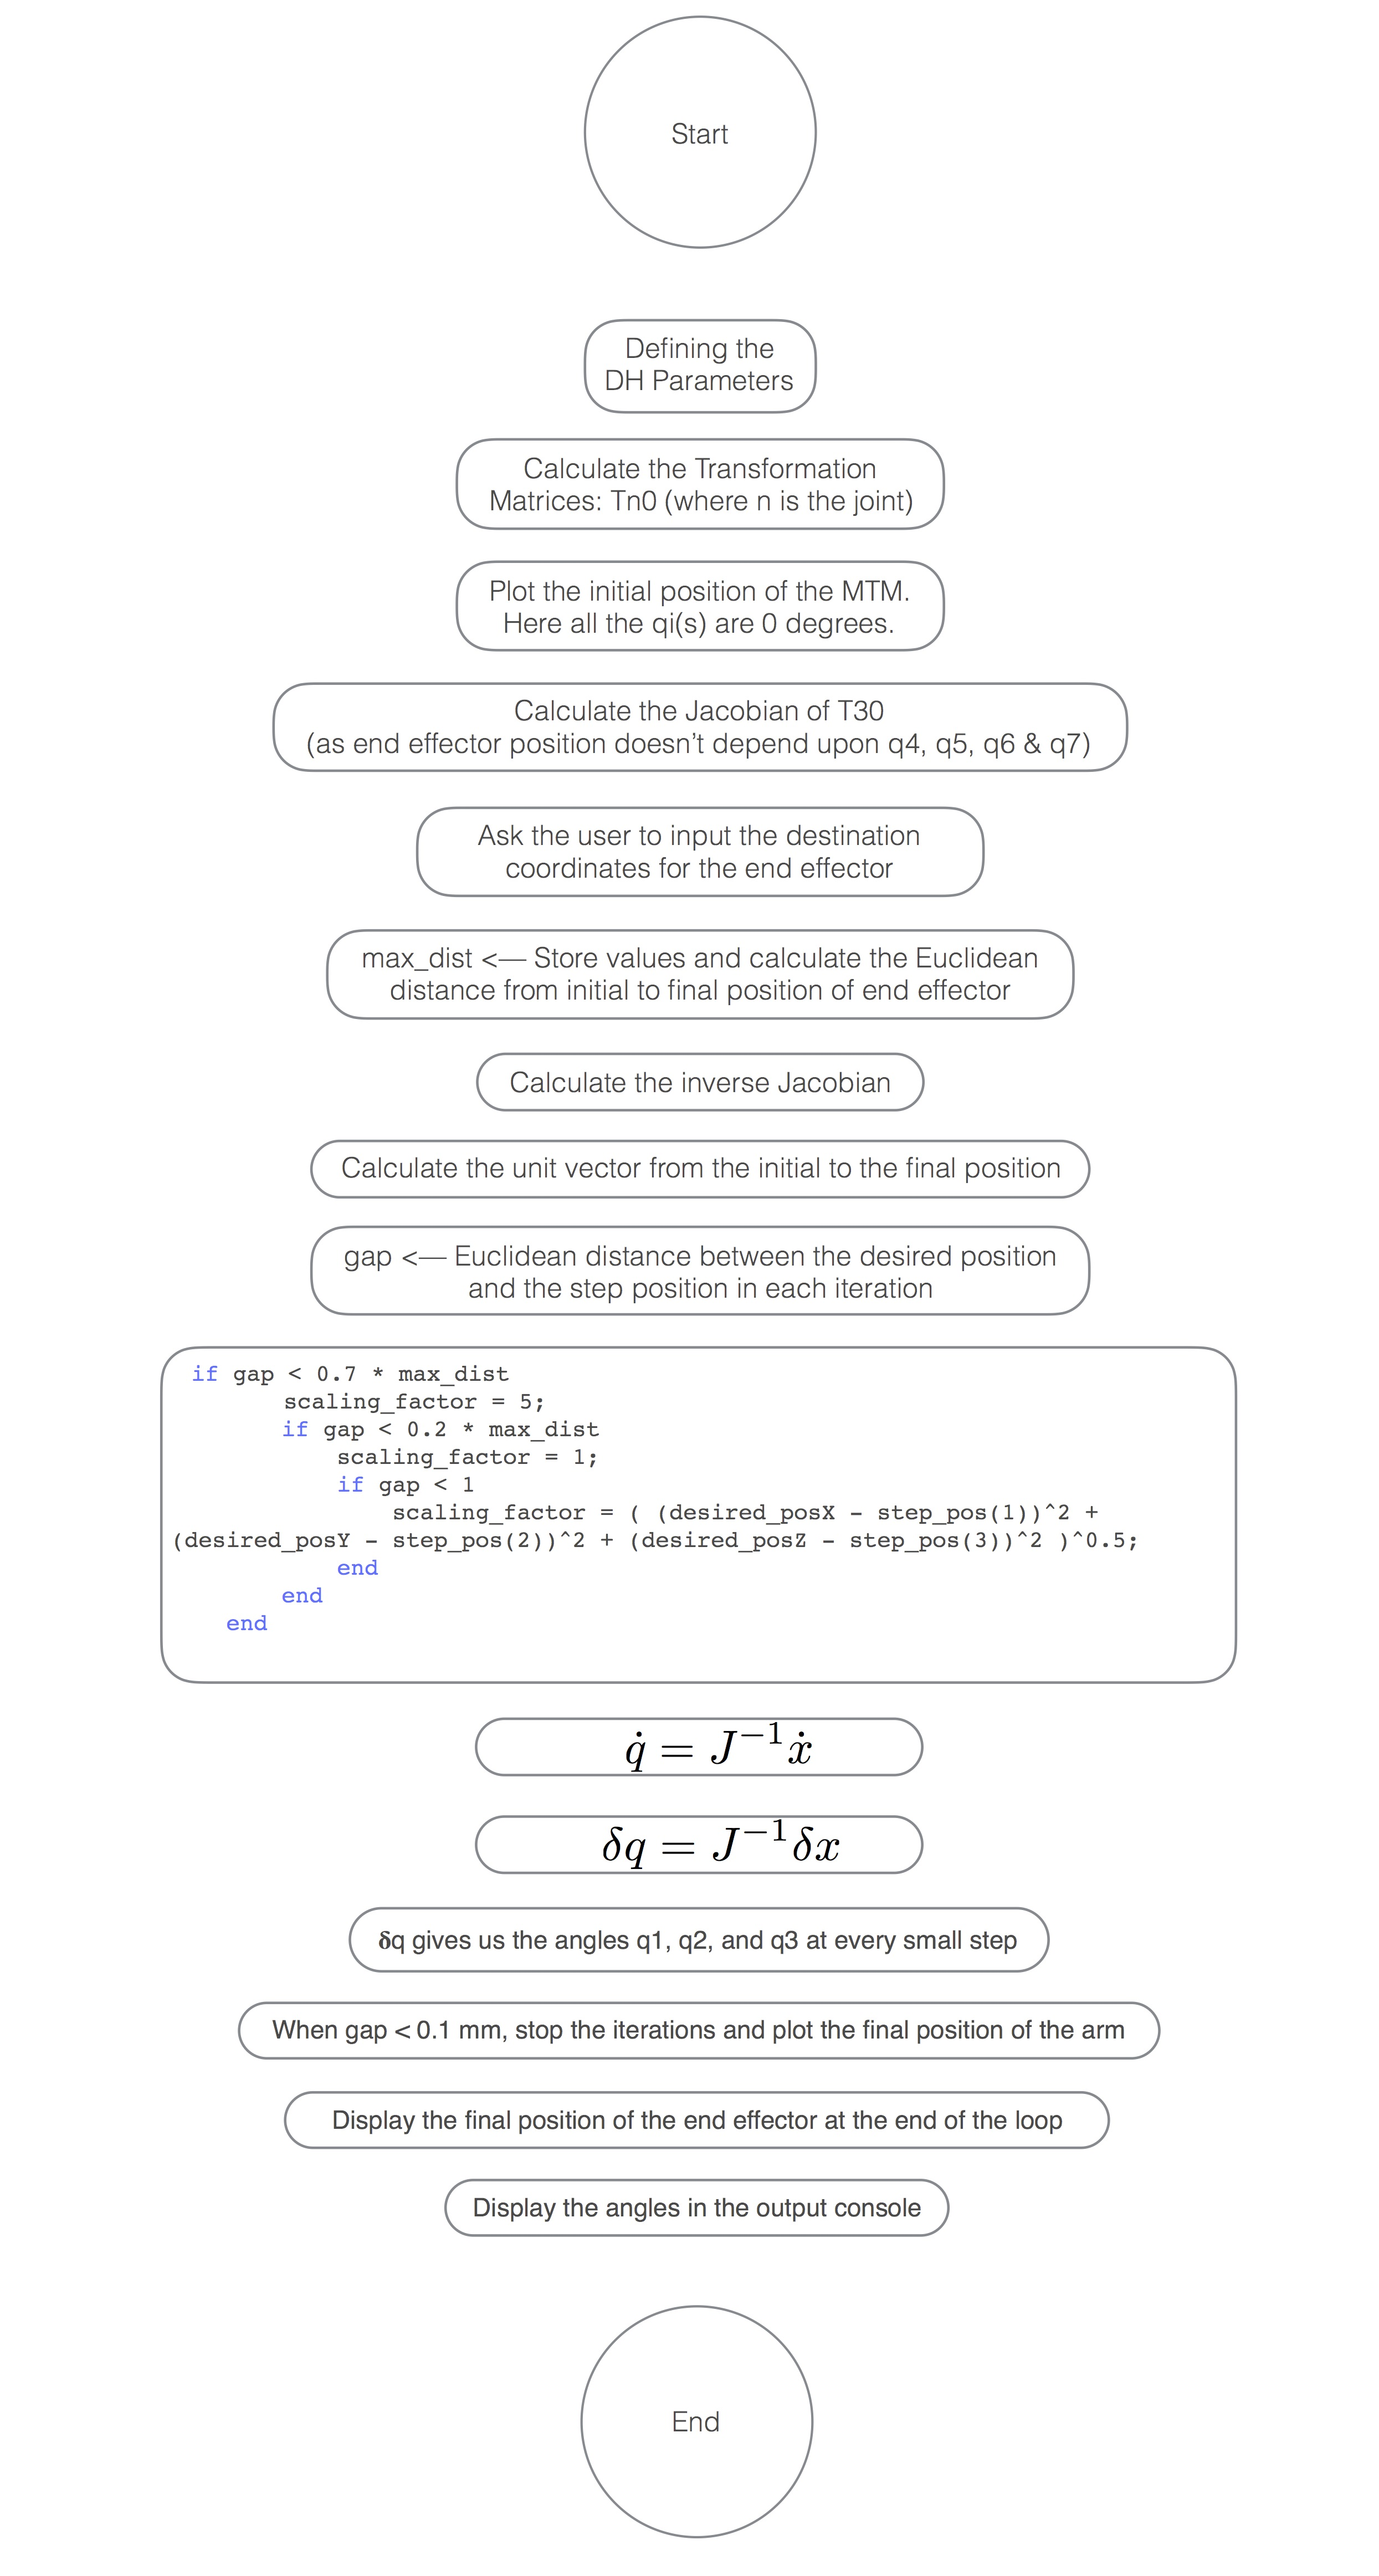
\includegraphics[width=3in, height=6in]{logicmtm.jpg}
\caption{: Steps to compute inverse kinematics for the MTM}
\label{fig:logicmtm}
\end{center}
\end{figure}

The forward kinematic method was used to validate the inverse kinematic computation. Forward kinematics were computed and implemented in Matlab using DH transformation matrix.
The plot in Figure~\ref{fig:plotpsm} shows the PSM in its home configuration in black with all its joint values set to 0 i.e. the configuration when there is no actuation. The position of the manipulator in this configuration is found using forward kinematics to be (0.43, -0.44, 0.00) and its Euler angles are found to be (0, 0, 0). The line plot in blue shows the PSM in its final configuration after performing forward kinematics with joint values obtained from the inverse kinematics for a desired position (0.5, -0.6, 0.2) and orientation specified by a set of Euler angles (0, 0, 0). As can be seen, the manipulator has been positioned correctly, while there are some glitches in getting the orientation to work properly. More details about inaccuracies in orientation are given in further plot descriptions.

\begin{figure}[htbp]
\begin{center}
\includegraphics[width=4in]{plotpsm.jpg}
\caption{: Plot of the PSM at its initial position}
\label{fig:plotpsm}
\end{center}
\end{figure}

The plot in Figure~\ref{fig:errorplot} indicates the change in orientation error with iterations. It is evident that the orientation error is an increasing sinusoid. The orientation error does not seem to converge and this again indicates a glitch in the computation. The position error however converges to zero relatively quickly (at the 47th iteration).

\begin{figure}[htbp]
\begin{center}
\includegraphics[width=3in]{errorplot.jpg}
\caption{: Plot of the PSM\textquotesingle s orientation and position errors vs. time (iterations)}
\label{fig:errorplot}
\end{center}
\end{figure}

The plot in Figure~\ref{fig:JointAnglesplot} shows the variation of joint angles with time or iterations. It can be inferred from the plot that joints 1, 2 and 3 converge to a stable value while joints 4, 5 and 5 do not. This again reinforces the fact that the positioning has been done correctly because joints 1, 2 and 3 are responsible for the positioning and joints 4, 5 and 6 are responsible for orienting the end effector. Here again, we see that joint values for joints 4, 5 and 6 is sinusoidal and the trend suggests that it is never converging to a bounded value.

\begin{figure}[htbp]
\begin{center}
\includegraphics[width=3in]{JointAnglesplot.jpg}
\caption{: Plot of the variation in joint angles with iterations}
\label{fig:JointAnglesplot}
\end{center}
\end{figure}

The plot in Figure~\ref{fig:JointPosTrackplot} shows the trajectories of all joints have been tracked in the task (Cartesian) space. Joints 1 and 2 are at the base and do not move and are hence not plotted. Joints 3 through 7 are plotted. It is interesting to observe the unstable behaviour of the system towards the end where the joints 4, 5 and 6 are used to orient the end effector towards the desired orientation. Until the curvy, unstable portion of the plot, the system seems to be stable i.e. when joints 1, 2 and 3 are performing the job of positioning the end effector to the desired position, there seems to be an almost straight line trajectory indicating stability and convergence towards the desired position.
Inverse kinematics for both MTM and PSM.

\begin{figure}[htbp]
\begin{center}
\includegraphics[width=3in]{JointPosTrackplot.jpg}
\caption{: Plot of joint trajectory tracking}
\label{fig:JointPosTrackplot}
\end{center}
\end{figure}

\section{Tasks Remaining}
In this section we shall describe the remaining tasks that needs to be completed for the project. The primary that remains to be completed in the project is to model an impedance controller and implement it in code. The steps to accomplish is shown in Figure~\ref{fig:comp_flow2}.

\begin{figure}[htbp]
\begin{center}
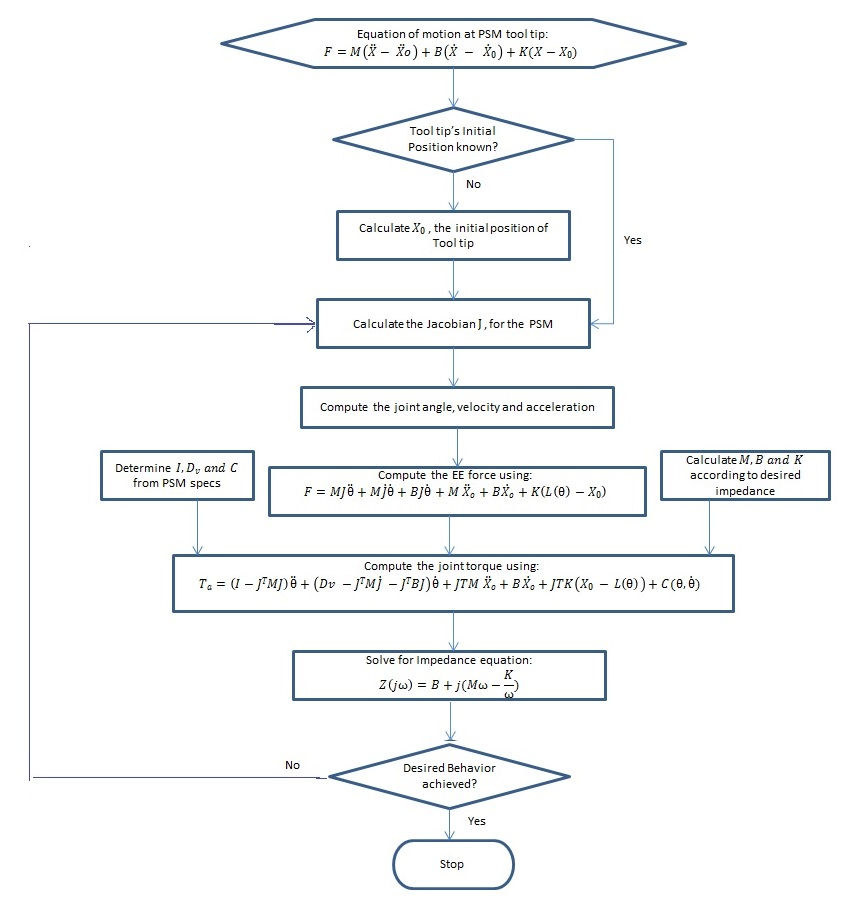
\includegraphics[width=3in,height=5in]{comp_flow2.jpg}
\caption{: Steps for computing an implementation of an impedance controller.}
\label{fig:comp_flow2}
\end{center}
\end{figure}

%\section{Conclusion}
%This section is for the conclusion.

\appendices

\section{Requirements Document}
In this section we shall define the requirements to develop an impedance control for the PSM tip.

\subsection{Unit Requirements}
\begin{itemize}
  \item The end effector position shall be represented in Cartesian coordinates.
  \item The joint parameters shall be represented in degrees.
  \item The forces shall be measured in N.
  \item The current shall be measured in milliamps.
\end{itemize}

\subsection{Functional Requirements}
\begin{itemize}
  \item The developed model shall be able to receive actual sensor data such as actuator (joint) position and current values from the joint actuator.
  \item The developed model shall be able to receive simulated sensor data for actuator position and joint actuator current.
  \item The developed model shall be able to receive simulated environmental force data at the PSM tip.
  \item The developed model shall be able to compute the joint kinematics and dynamics.
  \item The developed model shall be able to compute the end-effector position.
  \item The developed model shall be able to send computed positional information to the controller to position the PSM tip.
  \item The impedance controller shall implement the developed model to provide motion parameters as inputs for the manipulator and then generate the joint actuator forces based on the input parameters.
  \item User shall be able to programmatically control the motion of the manipulator in order to develop a dynamic relationship between the PSM end-effector position and the force.
\end{itemize}

\subsection{Non-functional Requirements}
\begin{itemize}
  \item The model shall be developed and implemented using ROS libraries provided by AIM Lab~\cite{aimlab} and JHU~\cite{dvrkjhu}.
  \item In the simulation the equations shall have to account for the frictional, inertial or gravitational dynamics of the manipulator but these can result in increasing the complexity of the controller~\cite{hogan1984}.
  \item The impedance control algorithm shall be built with terms to account for external disturbances~\cite{hogan1984}.
  \item The kinematic and dynamic model of all moving components shall be developed.
  \item The developed model shall define a static relation between the output force and the input displacement~\cite{hogan1984}.
\end{itemize}

\subsection{User Requirements}
\begin{itemize}
  \item The user shall have basic knowledge and understanding of robot parameters.
\end{itemize}

\subsection{Physical Requirements}
\begin{itemize}
  \item The actuators shall be capable of generating the commanded forces.
  \item The sensors shall be capable of monitoring the actuator position (or joint position in theta).
\end{itemize}

\subsection{Performance Requirements}
\begin{itemize}
  \item A maximum computational time of 1 millisecond per manipulator will be required for the information to go from the sensors to the higher system, such as a controller, and the resulting dynamics to take place.
  \item The PSM shall be able to maintain the slack on a piece of string whose one end is being held by the PSM tip and the other end being held and pulled by a human.
\end{itemize}

\section{DH Frame Assignments}

\begin{figure}[htbp]
\begin{center}
\includegraphics[width=3in]{dhframemtm.png}
\caption{: DH Frame Assignment for the MTM}
\label{fig:dhframemtm}
\end{center}
\end{figure}

\begin{figure}[htbp]
\begin{center}
\includegraphics[width=3in]{dhframepsm.png}
\caption{: DH Frame Assignment for the PSM}
\label{fig:dhframepsm}
\end{center}
\end{figure}


%\section{Inverse Kinematics - Matlab code}
%Appendix text goes here.

% Add references
\bibliographystyle{plain}
\bibliography{Bibliography}

\end{document}

